\documentclass[11pt]{article}
%ACENTOS
\usepackage[utf8]{inputenc}
\def\figurename{Fig.}
\def\tablename{Tabla}
\def\refname{Referencias}
\setlength{\parskip}{1em}

%PAQUETES
\usepackage{amsfonts,amsmath,amssymb}    % need for subequations
\usepackage{amsmath,latexsym}
\usepackage{graphics,color}
\usepackage{graphicx}
\usepackage{algpseudocode}
\usepackage[most]{tcolorbox}
\usepackage{hyperref} %Para colocar direcciones Web
\usepackage{booktabs} % Tablas
\usepackage[thinc]{esdiff} % Derivadas

%MARGEN
\setlength\topmargin{-0.5in}
\addtolength\oddsidemargin{-0.5in}
\setlength{\textheight}{23cm}
\setlength{\textwidth}{16cm}

%VARIABLES
\newcommand{\N}{\mathbb N}
\newcommand{\Z}{\mathbb Z}
\newcommand{\R}{\mathbb R}
\newcommand{\C}{\mathbb C}
\providecommand{\norm}[1]{\lVert#1\rVert}
%COLORES
\newcommand{\rojo}[1]{\textcolor[rgb]{1.00,0.00,0.00}{#1}}
\newcommand{\azul}[1]{\textcolor[rgb]{0.00,0.00,1.00}{#1}}
 
  
\begin{document}

\begin{center}
 \Large \underline {\\ \\Tarea 2: Ceros de funciones} \\ \medskip
 \small  {Elaborado por Giselt Parra}\\ 
 \footnotesize{Lunes, 26 de octubre de 2020.}
\end{center}


\begin{center} \Large {Propuestas} \end{center}

Con el fin de hacer el estudio de las propuestas planteadas para hallar ceros de funciones de manera ordenada, se ha decidido abordar las modificaciónes a los métodos involucrados por separado explicando las mejoras realizadas y así llegar a la propuesta final de manera incremental. 


\begin{center} \large {Métodos abiertos} \end{center}

La aproximación de los ceros de función en los métodos abiertos tales como el método de la Bisección y el método de Regula Falsi resulta ser lento. Como motivación para reducir el número de iteraciones necesarias para converger, se plantean estrategias para éstos métodos donde se reduce el entorno a hallar la raíz por cada iteración.

\vspace{0.5cm}
{\large (1) Método de la Bisección Mejorado}

Esta propuesta basa como mejora al método de la bisección segmentar el intervalo de entrada entre un número mayor a 2 y así cerrar de manera más rápida el entorno donde se encuentre la raiz por cada iteración.

%Sea n el número de subintervalos por el que queremos dividir en cada iteración % CHEQUEAR QUE SI CAMBIA EN NUMERO DE C ENTONCES PUEDE SER ALGO MAS

% CHEQUEEEEEEEEEAR 

%$$\lim_{k \to \infty}{\frac{|x_{k+1}-x_*|}{|x_k-x_*|}} = \frac{1}{n}$$


\vspace{0.25cm}	
\begin{center}
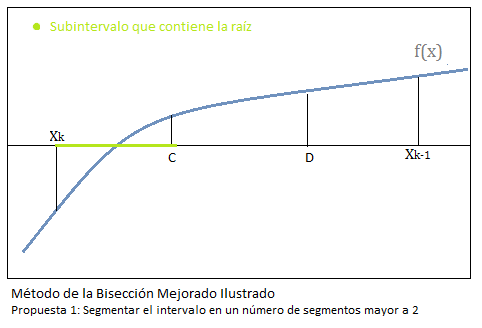
\includegraphics[keepaspectratio, width=8cm]{P11.png}
\end{center}
\vspace{0.25cm}


\vspace{0.5cm}
{\large (2) Método de Regula-Falsi Mejorado}

Consiste en combinar la idea de usar el punto medio c del intervalo en el que se está trabajando, tomar el subintervalo donde la gráfica corta con el eje x y la traza de una recta secante entre el punto (c, f(c)) y el otro punto extremo de dicho subintervalo.


\vspace{0.25cm}	
\begin{center}
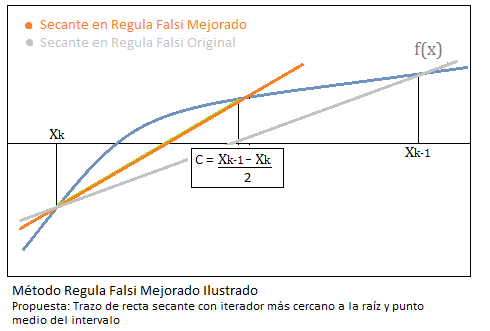
\includegraphics[keepaspectratio, width=8cm]{P2.png}
\end{center}
\vspace{0.25cm}


\vspace{0.5cm}
{\large (3) Método de la Bisección-Regula Falsi Mejorado}

En este método se integran las propuestas (1) y (3) en un solo método que permite hallar la raíz de la función segmentando el intervalo de entrada en tres subintervalos y trazando una recta secante entre uno de los extremos del subintervalo que contiene a la raíz con el punto medio de dicho subintervalo.

\vspace{0.25cm}	
\begin{center}
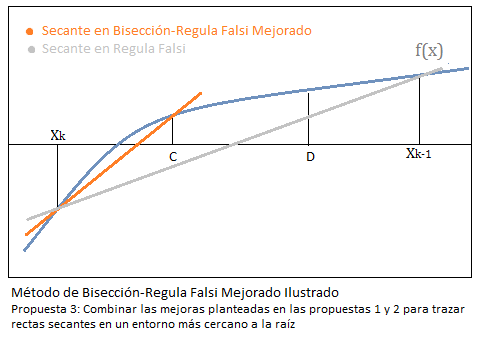
\includegraphics[keepaspectratio, width=8cm]{P3.png}
\end{center}
\vspace{0.25cm}



\begin{center} \large  {Resultados: Propuestas (1)(2)(3)} \end{center}

\begin{tcolorbox}[colframe=blue!35!black, title=Código]
    PropuestasMetodosAbiertos.m
\end{tcolorbox}

A continuación se muestra un cuadro comparativo de número de iteraciones requeridas por cada método para converger con la data de entrada correspondiente junto a la gráfica del residuo entre los métodos.

\begin{center}
    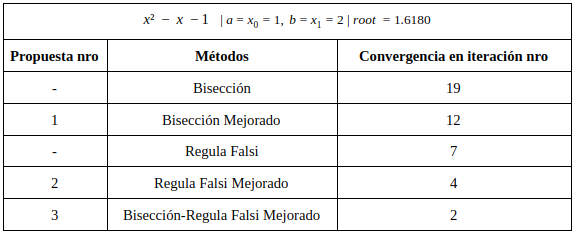
\includegraphics[keepaspectratio, width=10cm]{C1.png}
    \vspace{0.5cm}
    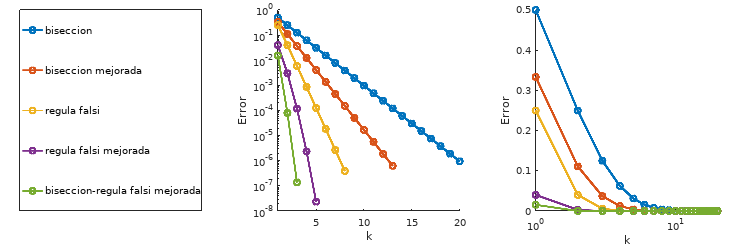
\includegraphics[keepaspectratio, width=14cm]{G1.png}
     \caption \tiny{\\ Prueba para la función $x^2 - x - 1$ donde la raíz se encuentra cerca del punto medio del intervalo [1,2]}
\end{center}  
\vspace{0.75cm}


\begin{center}
    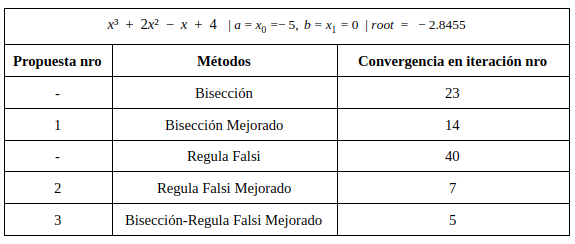
\includegraphics[keepaspectratio, width=10cm]{C2.png}
    \vspace{0.5cm}
    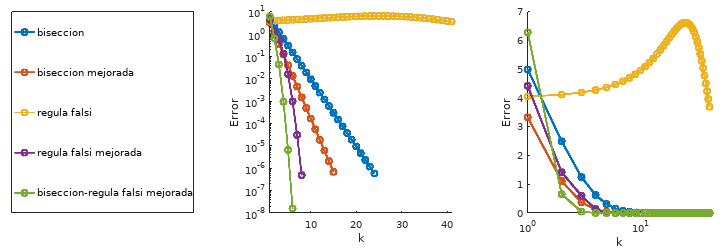
\includegraphics[keepaspectratio, width=14cm]{G2.png}
     \caption \tiny{\\ Prueba nro 1 para la función $x^3 + 2x^2 - x + 4$ en un intervalo amplio}
\end{center} 
Como se puede observar en los resultados para ésta ejecución, las mejoras realizadas al método de Regula Falsi hacen de este método no sólo más veloz sino también más robusto. Como se puede observar, el método Resula Falsi requiere un número mayor de iteraciones que el método de la Bisección. Esto se debe al comportamiento de la función en este intervalo, pues reduciendo el intervalo a la mitad genera mayor avance hacia la raíz que el corte de sucesivas rectas secantes dado a que cada nuevo iterador estará muy cerca del iterador actual. Al combinar las estrategias de convergencia entre estos dos métodos se da solución a este inconveniente en el método de Regula Falsi haciendolo más robusto.
\vspace{0.75cm}


\begin{center}
    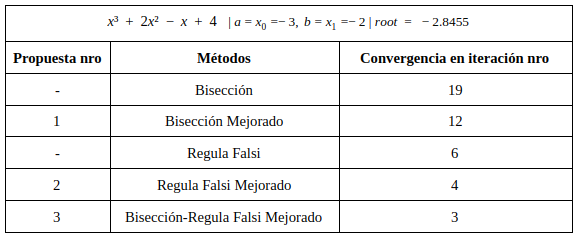
\includegraphics[keepaspectratio, width=10cm]{C3.png}
    \vspace{0.5cm}
    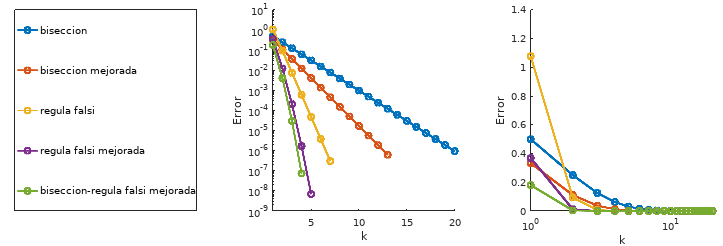
\includegraphics[keepaspectratio, width=14cm]{G3.png}
     \caption \tiny{\\ Prueba nro 2 para la función $x^3 + 2x^2 - x + 4$ en un intervalo más reducido}
\end{center} 

En conclusión, cada método mejorado arroja mejores resultados en velocidad de convergencia que el método anterior y los método originales expuestos en la Tarea 1 teniendo así el método de Bisección-Regula Falsi mejorado como el mayor velocidad de convergencia.

\vspace{0.75cm}


\begin{center} \large {Métodos cerrados} \end{center}


Se sabe que los métodos de Newton y Secante presentan la desventaja de que la convergencia es local y por tanto los iteradores iniciales deben estar lo suficientemente cerca de la raíz para alcanzar dicha convergencia. Uno de los caminos para usar estos métodos previniendo la no convergencia es haciendo uso de métodos abiertos para las primeras aproximaciones y así utilizar un método cerrado que llegará a la convergencia de manera más rápida una vez que el intervalo sea lo suficientemente pequeño. Es importante resaltar que este camino se propone como una solución en el cálculo univariable (caso escalar) dado a que la construcción de estos métodos como el método de la bisección resulta sencillo de construir. No ocurre lo mismo para el caso multivariable por tanto esta combinación de métodos abiertos con métodos cerrados no se extiende para mayor número de dimesiones, por tanto, existen otras alternativas que hacen de estos métodos cerrados más robustos y que podemos estudiar para hacer la respectiva analogía en el caso del cálculo univariable.

Existe un esquema de optimización para la búsqueda de puntos minimos en funciones. A estos esquemas se les conoce como algoritmos de descenso y consisten en hallar el cero del gradiente como la derivada multivariable de una función. Éste gradiente determina la pendiente hacia donde la función crece de manera más rápida, sin embargo, como el objetivo es hallar el mínimo se toma en sentido contrario, es decir, el método utiliza el negativo de la gradiente. Cada iteración de este esquema viene dado por: 
$$x_{k+1} = x_k + p_k s_k$$

donde $p_k$ es el gradiente negativo de la función y $s_k =\frac{f(x_k)}{f'(x_k)} $ que determina la longitud de paso. De este modo, la velocidad en la que los iteradores se aproximan a la raíz será mayor.

\vspace{0.5cm}

    
    
Como propuesta nro 4 ha sido el escogido el método de la secante siendo implementado con la estrategia antes expuesta en el método de Newton con la diferencia de prescindir de la derivada de la función y en reemplazo usar la formula de la recta secante. Junto a esta estrategia se integra la mejora planteada en la propuesta (3) para el método de Bisección y Regula Falsi.

\vspace{0.5cm}
{\large (4) Método de la Secante Mejorado}

Como ha sido mencionado previamente, para este método no se requiere la derivada de la función f. Sin embargo, éste método mejorado parte del siguiente razonamiento: 

$$f'(x) = \lim_{h \to 0}{\frac{f(x+h)-f(x)}{h}}$$

donde h será la longitud de los subintervalos generados luego de segmentar el intervalo entre los iteradores por un número grande. Ésta longitud será denominada $\Delta$. Considerando la expresión anterior y sabiendo que se está trabajando en un entorno cercano a la raíz se tiene que si $x_{k-1} - x_k \to 0$ entonces $\Delta \to 0$:

$$f'(x)	\approx \frac{f(x\pm\Delta)-f(x)}{\Delta}$$

Por lo que cada iterador nuevo será generado como

 $$x_{k+1} = x_k - \frac{f(x_k)}{ \frac{f(x_k\pm\Delta)-f(x_k)}{\Delta} } = 
  x_k - \frac{\Delta f(x_k)}{f(x_k\pm\Delta)-f(x_k)}
 \hspace{0.5cm} \forall k \in N$$ 

{\large Pasos a seguir por cada iteración k:}
\begin{enumerate}
	\item[\textperiodcentered] Evaluar los iteradores $x_k$ y $x_{k-1}$ en la función f para verificar el valor de las alturas en los respectivos puntos y seleccionar aquel cuya altura sea menor en magnitud.
	
\vspace{0.25cm}
\begin{center}
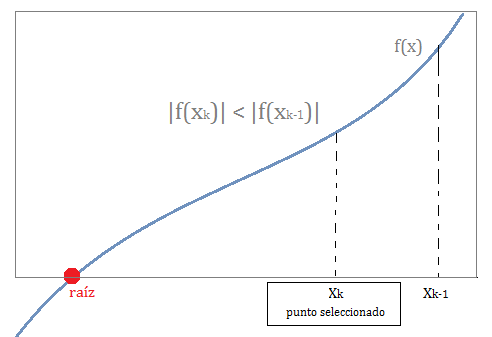
\includegraphics[keepaspectratio, width=8cm]{I.png}
\end{center}
\vspace{0.25cm}

	\item[\textperiodcentered] Se desea estimar en qué sentido se encuentra la raiz a hallar en la recta numérica. Para esto se tomará en cuenta el valor de los iteradores así como sus alturas. Por cada iteración y de esta forma se determinará si la raíz se encuentra hacia la derecha o hacia la izquierda del punto selecionado previamente.
	
\vspace{0.25cm}
\begin{center}
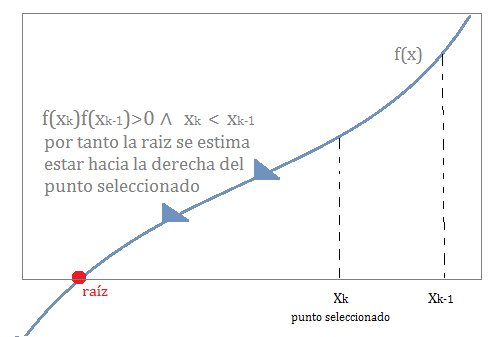
\includegraphics[keepaspectratio, width=8cm]{II.png}
\end{center}
\vspace{0.25cm}


	\item[\textperiodcentered] Segmentar el intervalo entre los iteradores e igualar $\Delta$ como la longitud de cada segmento.
	\item[\textperiodcentered] Se procede a trazar una recta secante con el punto seleccionado y este mismo desplazado $\Delta$ veces en el eje x. El desplazamiento del punto será en función de la dirección estimada de donde se encuentre la raíz.
	
\vspace{0.25cm}	
\begin{center}
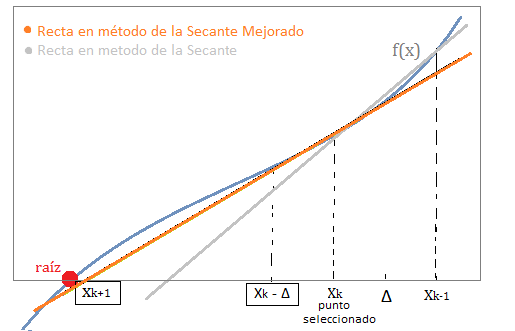
\includegraphics[keepaspectratio, width=8cm]{IIII.png}
\caption \tiny{\\Para ilustrar el funcionamiento del método y \\por simplicidad se segmentó el intervalo en dos}
\end{center}

\vspace{0.25cm}
         

	\item[\textperiodcentered] Se obtiene el siguiente iterador con el valor donde la recta secante trazada corta con el eje x y se repite este procedimiento hasta alcanzar la convergencia.

Consideraciones:
\\- Dado a que se evaluan las alturas de los iteradores en repetidas veces por cada iteración, éstas alturas serán evaluadas una sola vez al comienzo de la iteración con el propósito de optimizar el método en términos de ejecución. 
\\- Las modificaciones propuestas se orientan en el incremento de la velocidad de convergencia del método. Por lo tanto, los limitaciones en alcance persisten por lo que se debe garantizar las condiciones para la convergencia local del método original.

\end{enumerate}

\begin{center} \large  {Resultados: Propuesta (4)} \end{center}

\begin{tcolorbox}[colframe=blue!35!black, title=Código]
    PropuestaMetodoSecante.m
\end{tcolorbox}

A continuación se muestra un cuadro comparativo de número de iteraciones requeridas por cada método para converger con la data de entrada correspondiente junto a la gráfica del residuo entre los métodos.

\begin{center}
    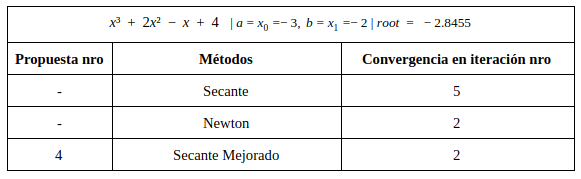
\includegraphics[keepaspectratio, width=10cm]{T1.png}
    \vspace{0.5cm}
    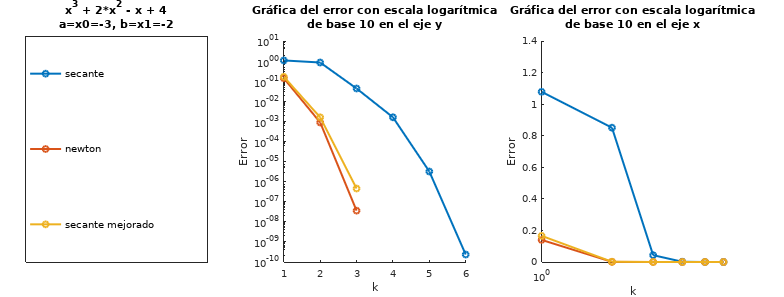
\includegraphics[keepaspectratio, width=14cm]{CL1.png}
    \caption \tiny{\\ Prueba nro 1 para la función $x^3 + 2x^2 - x + 4$ en un entorno cercano a la raíz}
    

\end{center}  
\vspace{0.75cm}


\begin{center}
    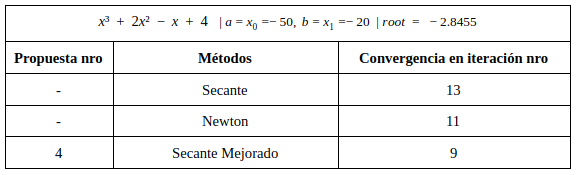
\includegraphics[keepaspectratio, width=10cm]{T2.png}
    \vspace{0.5cm}
    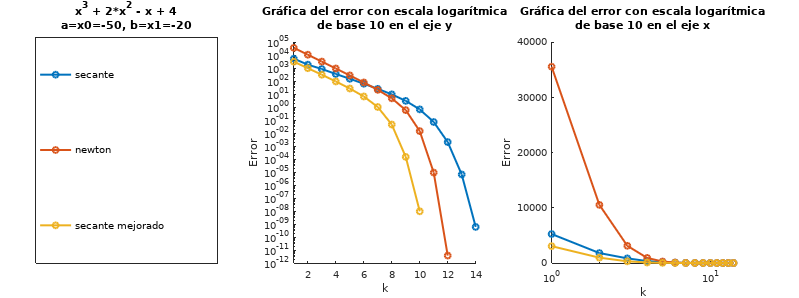
\includegraphics[keepaspectratio, width=14cm]{CL2.png}
     \caption \tiny{\\ Prueba nro 2 para la función $x^3 + 2x^2 - x + 4$ con iteradores iniciales lejanos a la raíz}

\end{center} 
\vspace{0.75cm}


\begin{center}
    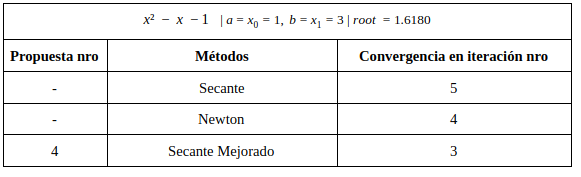
\includegraphics[keepaspectratio, width=10cm]{T3.png}
    \vspace{0.5cm}
    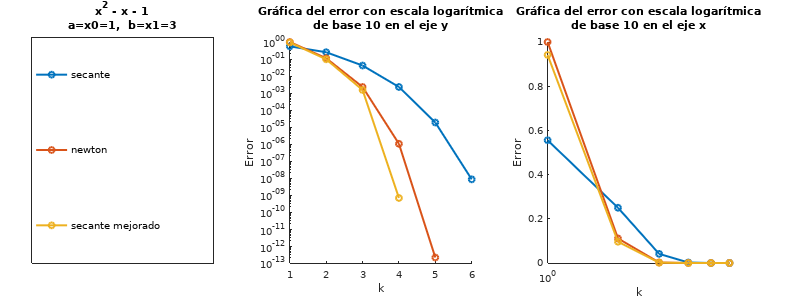
\includegraphics[keepaspectratio, width=14cm]{CL3.png}
    \caption \tiny{\\ Prueba para la función $x^2 - x - 1$}
\end{center} 
\vspace{0.75cm}    

Como se puede observar en los resultados, el método de la secante con las mejoras realizadas es capaz de alcanzar un desesmpeño en cuando a velocidad de convergencia casi tan bueno como el método original de Newton e incluso superandolo con la ventaja de ser menos costoso en cálculo por iteración y sin requerir de alguna otra función como lo es la derivada de la misma.


\begin{thebibliography}{9}
\bibitem{fi} 
Michael T. Heath. 
\textit{Scientific Computing: An Introductory Survey.}. 
University of Illinois at Urbana-Champaign, 1997.

\bibitem{se} 
Biswa N. Datta, Luis M. Hernández-Ramos y Marcos Raydan.
\textit{Análisis Numérico. Teoría y Práctica}. 
[2018]


\end{thebibliography}


\end{document}